%------------------------------------------------
% main.tex - Test document for LatexTree
%------------------------------------------------
\documentclass[12pt]{article}

% document info
\title{Test document}
\author{D Evans}
\date{June 2019}

% layout
\usepackage[margin=20mm, a4paper]{geometry}
\setlength{\parindent}{0ex}
\setlength{\parskip}{1ex}
%\pagestyle{plain}

% theorems
\usepackage{amsmath, amsthm}
\theoremstyle{plain}
\newtheorem{theo}{Theorem}%[section] 
\newtheorem{lem}[theo]{Lemma}
\theoremstyle{definition}
\newtheorem{defn}[theo]{Definition}
\theoremstyle{remark}
\newtheorem{rmk}[theo]{Remark}

% custom theorem style
\newtheoremstyle{mystyle}% name
{3pt}% space above
{3pt}% space below
{}% body font
{}% indent amount
{}% theorem head font
{.}% punctuation after theorem head
{.5em}% space after theorem head
{}% theorem head spec
\theoremstyle{mystyle}
\newtheorem{exc}[theo]{Exercise}

% dummy text
\usepackage{lipsum}

% hyperref
\usepackage{hyperref}
\hypersetup{colorlinks=true, linkcolor=blue}


% language declarations
\newcommand{\cy}{}
\newcommand{\en}{}
\newcommand{\bi}{}
%\usepackage[cy]{cambi}
 
% images
\usepackage{graphicx}
\graphicspath{{figures/}}
\usepackage{subfigure}
\renewcommand{\thefigure}{\thesection.\arabic{figure}}

% videos
\newcommand{\includevideo}[2][1]{\url{#2}}
%\usepackage{newfloat}
%\floatstyle{ruled}
%\DeclareFloatingEnvironment[
%    fileext=lov,
%    listname={List of Videos},
%    name=Video,
%    placement={!ht},
%    within=section
%]{video}
\usepackage{float}
\floatstyle{boxed}
\newfloat{video}{!ht}{lov}[section]
\floatname{video}{Video}
\usepackage{caption}
\captionsetup[video]{labelfont=normalfont}

% tweaks
\setcounter{tocdepth}{1}
\setcounter{secnumdepth}{5}


%----------------------------------------
\begin{document}%\label{doc:testdoc}
\maketitle
\tableofcontents

\begin{abstract}\noindent
\lipsum[2]
\end{abstract}

%--------------------
\section{Introduction}
\label{sec:intro}
This is a test file for \texttt{latextree.latex2html}.

% !TEX root = main.tex
\section{Sections}
\label{sec:sections}
\lipsum[1-1]

\subsection{A fancy title: $\alpha+\beta$}
\lipsum[2-2]

\section*{A section-level heading}
\lipsum[3-3]

\subsection*{A subsection-level heading}
\lipsum[4-4]


% !TEX root = main.tex
\section{Lists}

An unordered list:
\begin{itemize}
\item Apples\label{fru:afal}
\item Oranges\label{fru:oren}
\item Lemons
\end{itemize}

An unordered list with custom markers:
\begin{itemize}
\item[\bf ap] Apples
\item[$\alpha$] Oranges
\item[le] Lemons
\end{itemize}

An ordered list:
\begin{enumerate}
\item Cars
\item Buses
\item Bikes
\end{enumerate}

Nested enumerate lists
\begin{enumerate}
\item Cars
    \begin{enumerate}
    \item Ford
    \item Honda
    \end{enumerate}
\item Buses
    \begin{enumerate}
    \item Mini
    \item Coach
    \end{enumerate}
\item Bikes
    \begin{enumerate}
    \item Road
        \begin{enumerate}
        \item Racing
        \item Touring
        \end{enumerate}
    \item Mountain
    \end{enumerate}
\end{enumerate}


% !TEX root = main.tex

\section{Theorems}

\begin{defn}
This is a definition
\end{defn}

\begin{lem}[Zorn's lemma]
This is a lemma
\end{lem}

\begin{theo}
This is a theorem.
\begin{proof}
This is a proof
\end{proof}
\end{theo}

\begin{rmk}
This is a remark.
\end{rmk}

\begin{exc}
This is an exercise.
\end{exc}


%--------------------
\section{Boxes}

Here is a {\tt center} environment:
\begin{center}
Some text
\end{center}

A {\tt minipage} environment (these are inline environments):

\begin{minipage}{\linewidth}
Some text
\end{minipage}

A {\tt minipage} environment with a {\tt centering} declaration:

\begin{minipage}{\linewidth}
\centering
Some text
\end{minipage}

A {\tt minipage} environment with a {\tt raggedleft} declaration:

\begin{minipage}{\linewidth}
\raggedleft
Some text
\end{minipage}

%%--------------------
%\section{Tables}
%
%\subsection*{Inline}
%An inline \texttt{tabular} environment:
%\begin{tabular}{|ccc|}\hline
%$\alpha$ & $\beta$ & $\gamma$ \\ \hline
%$1/2$ & $1/3$ & $1/6$ \\ \hline
%\end{tabular}
%
%\subsection*{Centred}
%A centred \texttt{tabular} environment:
%\begin{center}
%\begin{tabular}{|c|c|c|}
%\hline
%a & b & c \\
%\hline
%d & e & f \\
%\hline
%\end{tabular}
%\end{center}
%
%\subsection*{Floats}
%A floating \texttt{table} environment:
%\begin{table}[htb]
%\centering
%\begin{tabular}{|c|c||c|c|c|} \hline
%Set Theory 		& 			& Logic			&		& \\ \hline
%Union			& $A\cup B$	& Disjunction 	& OR 	& $\lor$	\\
%Intersection		& $A\cap B$	& Conjunction	& AND 	& $\land$\\
%Complement		& $A^c$		& Negation		& NOT 	& $\lnot$	\\ \hline
%\end{tabular}
%\caption{Logic and Set Theory}
%\end{table}
%
% !TEX root = main.tex

\section{Mathematics}

An inline equation: $\sum_{n=1}^{\infty} a_n = 1$.

\bigskip
An \texttt{equation} environment:
\begin{equation}
\sum_{n=1}^{\infty} a_n = 1.
\end{equation}

An \texttt{equation*} environment:
\begin{equation*}
\sum_{n=1}^{\infty}\frac{1}{n^2} = \frac{\pi^2}{6}.
\end{equation*}

A \texttt{display} environment with LaTeX delimiters:
\[
x = \frac{-b\pm\sqrt{b^2-4ac}}{2a}.
\]

A \texttt{display} environment with TeX delimiters (double-dollars):
$$
x = \frac{-b\pm\sqrt{b^2-4ac}}{2a}.
$$

A \texttt{display} environment containing a \texttt{text} command, which itself contains (inline) mathmode:
\[
E=mc^2 \text{ where $c$ is the speed of light}.
\]

%--------------------
\subsection{Labelled equations}


An equation with a label:
\begin{equation}\label{eq:euler}
e^{i\pi}+1=0.
\end{equation}

Equation -\eqref{eq:euler}- is due to Euler.

An \texttt{align} environment:
\begin{align}\label{eq:polar}
x & = r\sin\theta \\
y & = r\cos\theta
\end{align}

%\bigskip
%A labelled \texttt{equation} environment:
%\begin{equation}\label{eq:einstein}
%E = mc^2
%\end{equation}
%Equation -\eqref{eq:einstein}- is due to AE. 

\bigskip
An {\tt equation} containing three {\tt pmatrix} environments:
\begin{equation}
\begin{pmatrix}0 & 1 \\ 1 & 0\end{pmatrix}
\qquad
\begin{pmatrix}0 & -i \\ i & 0\end{pmatrix}
\qquad
\begin{pmatrix}1 & 0 \\ 0 & -1\end{pmatrix}
\end{equation}


\section{\bf Text, \sl Text, \it Text \normalfont and \sc Text}

\subsection{Spacing problems}
Here is a sum $1+1=2$. Watch the comma $\sum x_n^2$, is there a space? Seems to be fixed!

\subsubsection*{Non-breaking spaces}
Tildes don't appear in mathmode. Here is an fbox containing lots of them:
\par
\fbox{$A~~~~~~~~~~~~~~~~~~~~~~~~~~~~~~~B$}
\par
This is useful to protect mathmode against VLE rewriters.


\subsection{Accents}
Delimited
\begin{itemize}
\item Not spaced: \'{e}\`{e}\^{w}\"{o}.
\item Spaced: \'{e} \`{e} \^{w} \"{o}.
\end{itemize}

Undelimited
\begin{itemize}
\item Not spaced: \'e\`e\^w\"o.
\item Spaced: \'e \`e \^w \"o.
\end{itemize}

Some words ...
\begin{itemize}
\item Cram\'{e}r-Rao.
\item Y m\^{o}r coch.
\end{itemize}

\subsection{Escaped characters}
\begin{itemize}
\item Not spaced: \&\%\$.
\item Spaced: \& \% \$ .
\end{itemize}	

We need to be careful with \$ characters!

\subsection{Font styles}
Here are some font styles: 
\begin{itemize}
\item \textbf{bold}
\item \textit{italic}
\item \texttt{teletype}
\item \textsc{small caps} 
\item \textsl{oblique}
\end{itemize}

%--------------------
\section{Declarations}

%--------------------
\subsection{Font style}
\label{ss:font-style-dec}

TeX-style teletype: {\tt LatexTree}.
\par
LaTeX-style teletype: \texttt{LatexTree}.

\begin{itemize}
\item No spaces: pre-{-inside-}-post
\item No spaces with TeX-style bold: pre-{-\bf bold-}-post
\end{itemize}

Remark: unlike Latex the browser compounds font styles:
\begin{itemize}
\item 
first {\tt second {\it third {\sc fourth} fifth} sixth} seventh
\end{itemize}
The browser renders `third' and `fifth' are shown in slanted teletype!

%--------------------
\subsection{Font size}
\label{ss:font-size-dec}

\begin{itemize}
\item \tiny tiny
\item \scriptsize scriptsize
\item \footnotesize footnotesize
\item \small small
\item \normalsize normalsize
\item \large large
\item \Large Large
\item \LARGE LARGE
\item \huge huge
\item \Huge Huge
\end{itemize}
\normalsize

%\tiny{tiny}, \scriptsize{scriptsize}, \footnotesize{footnotesize}, \small{small}, \normalsize{normalsize}, \large{large}, \Large{Large}, \LARGE{LARGE}, \huge{huge}, \Huge{Huge}.
%\normalsize

All declarations have (inline) environments of the same name:

For example 
\begin{small}
small
\end{small}
and
\begin{large}
large.
\end{large}

%--------------------
\subsection{Language declarations}
\label{ss:language-dec}

pre-{-normal \bf bold \it italic \normalfont normal-}-post

pre-{-common \cy cymraeg \en english \bi common-}-post 



%--------------------
\section{Links}
\label{sec:links}

Here is a labelled theorem containing a labelled equation.
\begin{theo}[Pythagoras' Theorem]\label{thm:pythagoras}
\begin{equation}\label{eq:pythagoras}
a^2 + b^2 = c^2.
\end{equation}
\end{theo}

% Labels are attached to the parent environment or block. 
% A second label will overwrite the first.
\subsection{Cross-references}
\label{ss:xrefs}
\begin{itemize}
\item Here is a ref -\ref{sec:intro}- to the introduction.
\item Here is a ref -\ref{sec:links}- to the current section.
\item Here is a ref -\ref{ss:xrefs}- to the current subsection.
\item Here is a ref -\ref{thm:pythagoras}- to the above theorem.
\item Here is an eqref -\eqref{eq:pythagoras}- to the equation in the above theorem.
\end{itemize}

\subsection{Citations}
\begin{itemize}
\item A citation -\cite{grimmett01}- to the first bibtex entry.
\item A citation -\cite{hogg05}- to the second bibtex entry.
\item A citation -\cite{grimmett01,hogg05}- to the first two bibtex entries.
\end{itemize}

\subsection{The hyperref package}
\begin{itemize}
\item Here is a url: -\url{http://www.bbc.co.uk/}-.
\item Here is some -\href{http://www.bbc.co.uk/}{hyperlinked text}-.
\item Here is a -\hyperref[sec:intro]{named cross-reference}- to the introduction.
\item here is an autoref -\autoref{sec:intro}- to the introduction.
\item Here is a nameref -\nameref{sec:intro}- to the introduction.
\end{itemize}

\subsection*{Document-level labels}
For a viewable links to the document-level label we need to use the \texttt{hyperref} command as follows: -\hyperref[doc:testdoc]{back-to-top}-. There is no number or title associated with the document-level so other xref commands don't know what to display. Document-level labels might be useful to organise documents within and across modules.

%--------------------
% Latex creates a "References" heading automatically
\begin{thebibliography}{1}
\bibitem{grimmett01}
Geoffrey R. Grimmett and David R. Stirzaker.
\newblock {\em Probability and Random Processes}.
\newblock Oxford University Press, third edition, 2001.
\bibitem{hogg05}
Robert V. Hogg, Joseph W. McKean and Allen T. Craig.
\newblock {\em Introduction to Mathematical Statistics}.
\newblock Prentice Hall, sixth edition, 2005.
\end{thebibliography}



%--------------------
\section{Counters}
%\renewcommand{\thetheorem}{\alph{theorem}}
\begin{itemize}
\item \Alph{section}
\item \arabic{theo}
\item \Roman{equation}
\end{itemize}

%--------------------
\section{Verbatim}
pre
\begin{verbatim}
Say \hello wave \goodbye ...
class A():
	pass
class B(A):
	pass
\end{verbatim}
post

%\newcounter{rhestr}
%\newcounter{eitem}%[rhestr] % numbered within aka reset
%
%%\numberwithin{eitem}{rhestr}
%\counterwithin{eitem}{rhestr}
%\renewcommand{\theeitem}{\therhestr.\roman{eitem}}
%
%\stepcounter{rhestr}
%\setcounter{eitem}{3}
%\stepcounter{rhestr}
%\stepcounter{eitem}
%\begin{itemize}
%\item \therhestr
%\item \theeitem
%\end{itemize}

%--------------------
\section{Videos}
Embedding videos in PDFs is difficult, and it's better to include hyperlinks to YouTube videos using the \texttt{url} and \texttt{href} commands. 


\subsection*{\texttt{url} commands}
Please watch this video: \url{https://www.youtube.com/watch?v=oCDXhvXye9E}.

\subsection*{\texttt{href} commands}
Please watch this \href{https://www.youtube.com/watch?v=oCDXhvXye9E}{video}.

\subsection{\texttt{video} environments}
We define a new float called {\tt video} which uses the custom {\tt includevideo} command. This command is intended to mirror the way that {\tt includegraphics} is used within {\tt figure} floats. In the PDF version this is again rendered as a hyperlink, but {\tt LatexTree} embeds the video into the webpage.

Why does it need to be a {\tt float} instead of a simple environment?

\par\qquad -- For PDF it's simply a centred/displayed URL in Latex (one line).
\par\qquad -- For HTML there's no need to float it!

However it gives displayed videos the look and feel of figures and tables in terms of boxed, captions, etc. and we can have {\tt lov} too.

\paragraph*{Note} To get an embed code for a YouTube video, click on {\tt Share->Embed} under the video and it will generate an entire {\tt iframe} tag from which the URL can be easily recovered.

\begin{video}
\centering
\includevideo[scale=0.5]{https://www.youtube.com/embed/oCDXhvXye9E}
\caption{Listen and learn folks!\label{vid:orange}}
\end{video}

\appendix
\section{Jobs List}
\begin{itemize}
\item MC/MA as forms
\item Table of contents
\item Images and videos
\item Numerals
\end{itemize}

%\section{Remarks}
%For a particular bibitem the cite-key behaves exactly like a label (for that bibitem) and cite commands act exactly like ref commands, so we could just add these to the xref-table: cite-key mapped to this bibitem. The cite-key should be assigned as a attribute of this bibitem (which is a block command ie. a container) so URLs placed into cite elements point to the item itself (rather than the bibliography itself).

\section{Figures}

We parse the optional argument to \texttt{includegraphics}. The \texttt{Image} class has an attribute \texttt{width} expressed as a percentage. This is computed from the (optional) \texttt{scale} or \texttt{width} parameters passed to \texttt{includegraphics}.

\begin{itemize}
\item \autoref{fig:acapb} is the original (scale = 0.25).
\item \autoref{fig:acapb-big} is the big one (scale = 0.5).
\item \autoref{fig:acapb-small} is the small one (scale = 0.1).
\item \autoref{fig:setops-subfig} shows a figure layout using \texttt{subfigure}.
\item \autoref{fig:setops-tabular} shows a figure layout using \texttt{tabular}. %The optional parameter to \texttt{includegraphics} is \texttt{scale=0.4}, and the pictures take up 40\% of each cell, which is a pity.
\end{itemize}

\begin{figure}[ht]
\centering
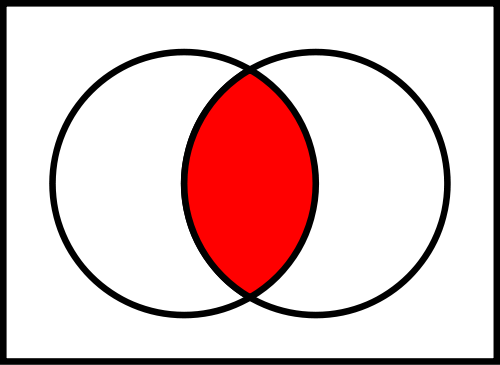
\includegraphics[scale=0.25]{AcapB}
\caption{Set intersection (scale=0.25)\label{fig:acapb}}
\end{figure}

\begin{figure}[ht]
\centering
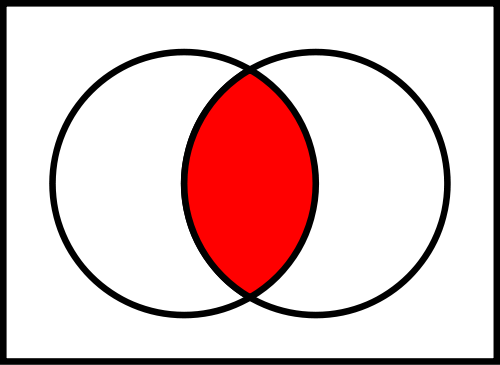
\includegraphics[scale=0.5]{AcapB}
\caption{The big one (scale=0.5)\label{fig:acapb-big}}
\end{figure}

\begin{figure}[ht]
\centering
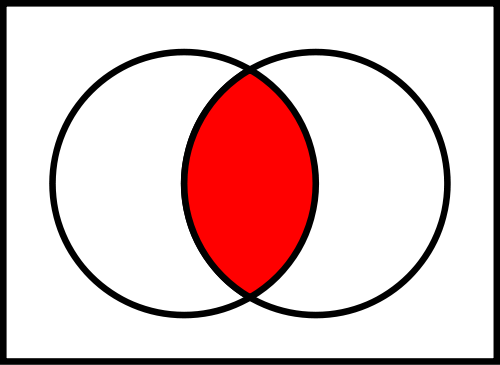
\includegraphics[scale=0.1]{AcapB}
\caption{The small one (scale=0.1)\label{fig:acapb-small}}
\end{figure}

\begin{figure}[ht]
\centering
\subfigure[Union]{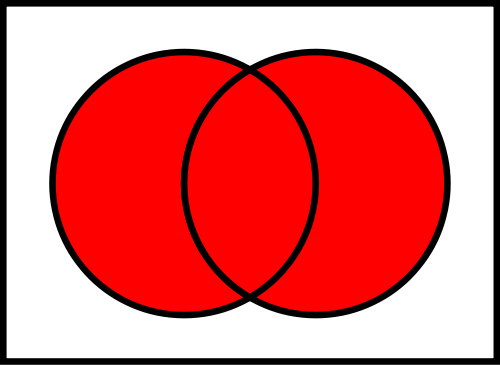
\includegraphics[scale=0.25]{AcupB}\label{fig:union}}
\subfigure[Intersection]{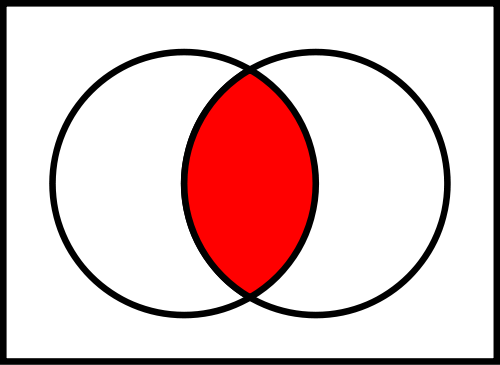
\includegraphics[scale=0.25]{AcapB}\label{fig:intersection}}
\subfigure[Complement]{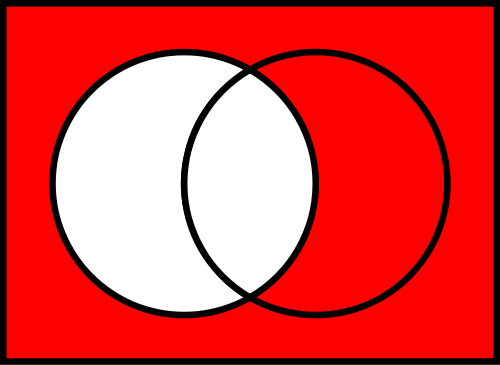
\includegraphics[scale=0.25]{Acomp}\label{fig:complement}}
\caption{Three figures using \texttt{subfigure}.\label{fig:setops-subfig}}
\end{figure}

%\begin{figure}
%\centering
%\begin{tabular}{ccc}
%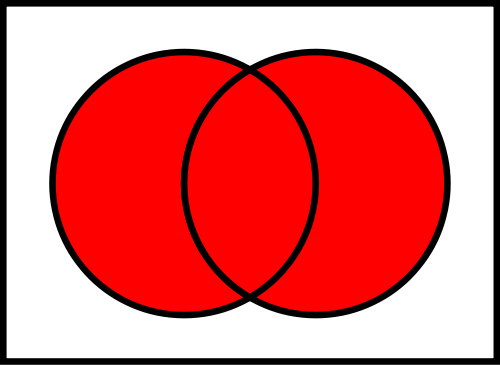
\includegraphics[width=0.25\linewidth]{AcupB} &
%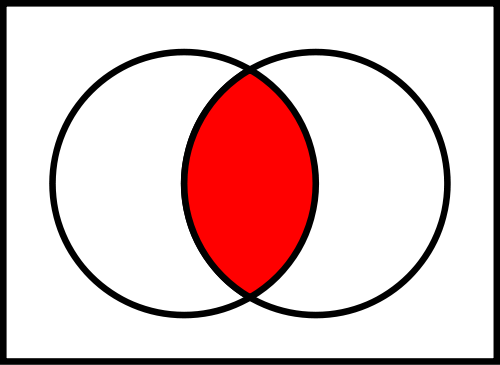
\includegraphics[width=0.25\textwidth]{AcapB} &
%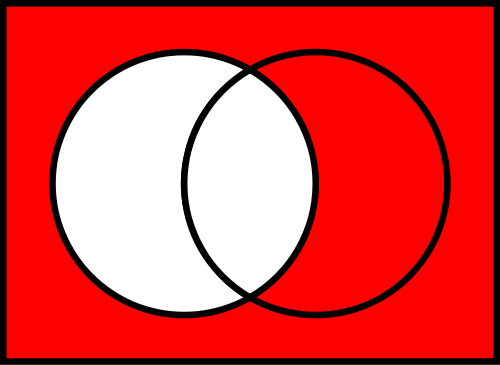
\includegraphics[width=0.25\textwidth]{Acomp} \\
%(a) Union & (b) Intersection & (c) Complementation \\
%\end{tabular}
%\caption{Three figures using \texttt{tabular}.\label{fig:setops-tabular}}
%\end{figure}

%=====================================================================
\cleardoublepage
\newpage
%\counterwithin{figure}{section}
%\counterwithout{figure}{section}

\section{Testbed}
%=====================================================================
\begin{figure}[ht]
\centering
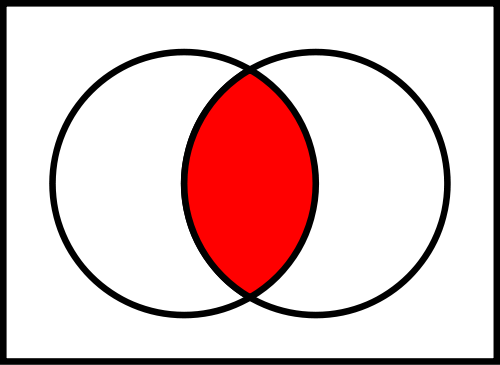
\includegraphics[scale=0.25]{AcapB}
%\caption{Set intersection\label{fig:acapb}}
\end{figure}

\begin{figure}[ht]
\centering
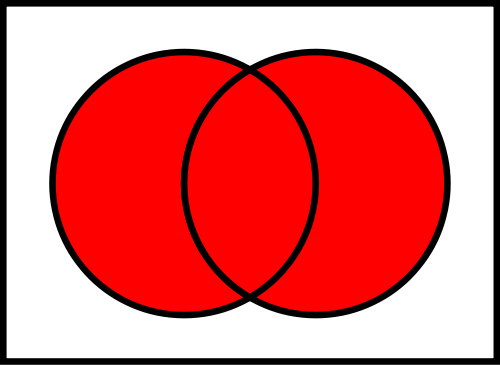
\includegraphics[scale=0.25]{AcupB}
\caption{Set union\label{fig:acupb}}
\end{figure}

Multiple captions:
\begin{figure}[ht]
\centering
\caption{Above above?}
\caption*{Above?}
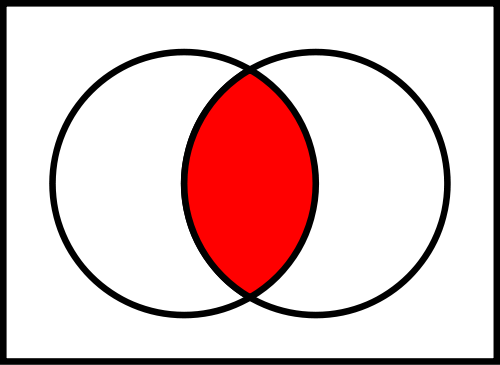
\includegraphics[scale=0.25]{AcapB}
\caption[lot]{Set intersection\label{fig:acapb}}
\end{figure}



%=====================================================================
\end{document}